\documentclass[12pt,a4paper]{article}
\usepackage{fontspec,graphicx,caption}
\usepackage[left=4cm,right=3cm,top=3cm,bottom=3cm]{geometry}
\setmainfont{Times New Roman}
\setlength{\parindent}{0pt}
\captionsetup{font=small,labelformat=empty}
\begin{document}
\noindent\includegraphics[width=14cm]{../bab6/00_distribution_total_as_ass.pdf}
\captionof{figure}{Distribusi Wrong/Acceptable/Abstain/Missing pada Asia Selatan–Afrika Sub-Sahara, penyebut seluruh respons. Wrong berarti keputusan tindakan salah, bukan jawaban model salah. AS = Asia Selatan; ASS = Afrika Sub-Sahara.}
\clearpage
\noindent\includegraphics[width=14cm]{../bab6/00_distribution_total_au_at.pdf}
\captionof{figure}{Distribusi Wrong/Acceptable/Abstain/Missing pada Amerika Utara–Asia Timur, penyebut seluruh respons. Wrong berarti keputusan tindakan salah, bukan jawaban model salah. AU = Amerika Utara; AT = Asia Timur.}
\clearpage
\noindent\includegraphics[width=14cm]{../bab6/04_reasons_abstain_as_ass_1.pdf}
\captionof{figure}{Alasan abstain pada Asia Selatan–Afrika Sub-Sahara, kelompok model 1/2. Persentase dari n respons abstain per skenario (empat subset); skala 0–100\%. AS = Asia Selatan; ASS = Afrika Sub-Sahara.}
\clearpage
\noindent\includegraphics[width=14cm]{../bab6/04_reasons_abstain_as_ass_2.pdf}
\captionof{figure}{Alasan abstain pada Asia Selatan–Afrika Sub-Sahara, kelompok model 2/2. Persentase dari n respons abstain per skenario (empat subset); skala 0–100\%. AS = Asia Selatan; ASS = Afrika Sub-Sahara.}
\clearpage
\noindent\includegraphics[width=14cm]{../bab6/04_reasons_abstain_au_at_1.pdf}
\captionof{figure}{Alasan abstain pada Amerika Utara–Asia Timur, kelompok model 1/2. Persentase dari n respons abstain per skenario (empat subset); skala 0–100\%. AU = Amerika Utara; AT = Asia Timur.}
\clearpage
\noindent\includegraphics[width=14cm]{../bab6/04_reasons_abstain_au_at_2.pdf}
\captionof{figure}{Alasan abstain pada Amerika Utara–Asia Timur, kelompok model 2/2. Persentase dari n respons abstain per skenario (empat subset); skala 0–100\%. AU = Amerika Utara; AT = Asia Timur.}
\clearpage
\noindent\includegraphics[width=14cm]{../bab6/06_accuracy_committed_as_ass.pdf}
\captionof{figure}{Akurasi committed pada Asia Selatan–Afrika Sub-Sahara, per subset. Penyebut: committed; c menunjukkan commit rate terhadap seluruh respons. AS = Asia Selatan; ASS = Afrika Sub-Sahara.}
\clearpage
\noindent\includegraphics[width=14cm]{../bab6/06_accuracy_committed_au_at.pdf}
\captionof{figure}{Akurasi committed pada Amerika Utara–Asia Timur, per subset. Penyebut: committed; c menunjukkan commit rate terhadap seluruh respons. AU = Amerika Utara; AT = Asia Timur.}
\clearpage
\noindent\includegraphics[width=14cm]{../bab6/11_conditional_accuracy_as_ass.pdf}
\captionof{figure}{Delta akurasi persona−N pada Asia Selatan–Afrika Sub-Sahara, dalam poin persentase; pasangan sama-sama committed. Bintang: Exact McNemar setelah Holm <0,05, keluarga 16. AS = Asia Selatan; ASS = Afrika Sub-Sahara.}
\clearpage
\noindent\includegraphics[width=14cm]{../bab6/11_conditional_accuracy_au_at.pdf}
\captionof{figure}{Delta akurasi persona−N pada Amerika Utara–Asia Timur, dalam poin persentase; pasangan sama-sama committed. Bintang: Exact McNemar setelah Holm <0,05, keluarga 16. AU = Amerika Utara; AT = Asia Timur.}
\clearpage
\noindent\includegraphics[width=14cm]{../pelengkap/05_reasons_nonmissing_as_ass_1.pdf}
\captionof{figure}{Alasan abstain pada Asia Selatan–Afrika Sub-Sahara, kelompok model 1/2. Persentase dari n respons nonmissing per skenario (empat subset); skala 0–100\%. AS = Asia Selatan; ASS = Afrika Sub-Sahara.}
\clearpage
\noindent\includegraphics[width=14cm]{../pelengkap/05_reasons_nonmissing_as_ass_2.pdf}
\captionof{figure}{Alasan abstain pada Asia Selatan–Afrika Sub-Sahara, kelompok model 2/2. Persentase dari n respons nonmissing per skenario (empat subset); skala 0–100\%. AS = Asia Selatan; ASS = Afrika Sub-Sahara.}
\clearpage
\noindent\includegraphics[width=14cm]{../pelengkap/05_reasons_nonmissing_au_at_1.pdf}
\captionof{figure}{Alasan abstain pada Amerika Utara–Asia Timur, kelompok model 1/2. Persentase dari n respons nonmissing per skenario (empat subset); skala 0–100\%. AU = Amerika Utara; AT = Asia Timur.}
\clearpage
\noindent\includegraphics[width=14cm]{../pelengkap/05_reasons_nonmissing_au_at_2.pdf}
\captionof{figure}{Alasan abstain pada Amerika Utara–Asia Timur, kelompok model 2/2. Persentase dari n respons nonmissing per skenario (empat subset); skala 0–100\%. AU = Amerika Utara; AT = Asia Timur.}
\clearpage
\noindent\includegraphics[width=14cm]{../pelengkap/07_effective_success_rate_nonmissing_as_ass.pdf}
\captionof{figure}{Keberhasilan efektif pada Asia Selatan–Afrika Sub-Sahara, per subset. Penyebut: nonmissing; c menunjukkan commit rate terhadap seluruh respons. AS = Asia Selatan; ASS = Afrika Sub-Sahara.}
\clearpage
\noindent\includegraphics[width=14cm]{../pelengkap/07_effective_success_rate_nonmissing_au_at.pdf}
\captionof{figure}{Keberhasilan efektif pada Amerika Utara–Asia Timur, per subset. Penyebut: nonmissing; c menunjukkan commit rate terhadap seluruh respons. AU = Amerika Utara; AT = Asia Timur.}
\clearpage
\noindent\includegraphics[width=14cm]{../pelengkap/08_pct_answer_wrong_as_ass.pdf}
\captionof{figure}{Keputusan Wrong pada Asia Selatan–Afrika Sub-Sahara, per subset. Penyebut: committed; c menunjukkan commit rate terhadap seluruh respons. AS = Asia Selatan; ASS = Afrika Sub-Sahara.}
\clearpage
\noindent\includegraphics[width=14cm]{../pelengkap/08_pct_answer_wrong_au_at.pdf}
\captionof{figure}{Keputusan Wrong pada Amerika Utara–Asia Timur, per subset. Penyebut: committed; c menunjukkan commit rate terhadap seluruh respons. AU = Amerika Utara; AT = Asia Timur.}
\clearpage
\noindent\includegraphics[width=14cm]{../pelengkap/10_coverage_as_ass_1.pdf}
\captionof{figure}{Delta commit rate persona−N pada Asia Selatan–Afrika Sub-Sahara, dalam poin persentase; pasangan nonmissing. Bintang: Exact McNemar setelah Holm <0,05, keluarga 16. AS = Asia Selatan; ASS = Afrika Sub-Sahara.}
\clearpage
\noindent\includegraphics[width=14cm]{../pelengkap/10_coverage_as_ass_2.pdf}
\captionof{figure}{Delta commit rate persona−N pada Asia Selatan–Afrika Sub-Sahara, dalam poin persentase; pasangan nonmissing. Bintang: Exact McNemar setelah Holm <0,05, keluarga 16. AS = Asia Selatan; ASS = Afrika Sub-Sahara.}
\clearpage
\noindent\includegraphics[width=14cm]{../pelengkap/10_coverage_au_at_1.pdf}
\captionof{figure}{Delta commit rate persona−N pada Amerika Utara–Asia Timur, dalam poin persentase; pasangan nonmissing. Bintang: Exact McNemar setelah Holm <0,05, keluarga 16. AU = Amerika Utara; AT = Asia Timur.}
\clearpage
\noindent\includegraphics[width=14cm]{../pelengkap/10_coverage_au_at_2.pdf}
\captionof{figure}{Delta commit rate persona−N pada Amerika Utara–Asia Timur, dalam poin persentase; pasangan nonmissing. Bintang: Exact McNemar setelah Holm <0,05, keluarga 16. AU = Amerika Utara; AT = Asia Timur.}
\clearpage
\noindent\includegraphics[width=14cm]{../pelengkap/12_effective_success_as_ass.pdf}
\captionof{figure}{Delta keberhasilan efektif persona−N pada Asia Selatan–Afrika Sub-Sahara, dalam poin persentase; pasangan nonmissing. Bintang: Exact McNemar setelah Holm <0,05, keluarga 16. AS = Asia Selatan; ASS = Afrika Sub-Sahara.}
\clearpage
\noindent\includegraphics[width=14cm]{../pelengkap/12_effective_success_au_at.pdf}
\captionof{figure}{Delta keberhasilan efektif persona−N pada Amerika Utara–Asia Timur, dalam poin persentase; pasangan nonmissing. Bintang: Exact McNemar setelah Holm <0,05, keluarga 16. AU = Amerika Utara; AT = Asia Timur.}
\clearpage
\noindent\includegraphics[width=14cm]{../pelengkap/13_stance_wrong_as_ass.pdf}
\captionof{figure}{Delta proporsi Wrong persona−N pada Asia Selatan–Afrika Sub-Sahara, dalam poin persentase; pasangan sama-sama committed. Bintang: Exact McNemar setelah Holm <0,05, keluarga 16. AS = Asia Selatan; ASS = Afrika Sub-Sahara.}
\clearpage
\noindent\includegraphics[width=14cm]{../pelengkap/13_stance_wrong_au_at.pdf}
\captionof{figure}{Delta proporsi Wrong persona−N pada Amerika Utara–Asia Timur, dalam poin persentase; pasangan sama-sama committed. Bintang: Exact McNemar setelah Holm <0,05, keluarga 16. AU = Amerika Utara; AT = Asia Timur.}
\clearpage
\noindent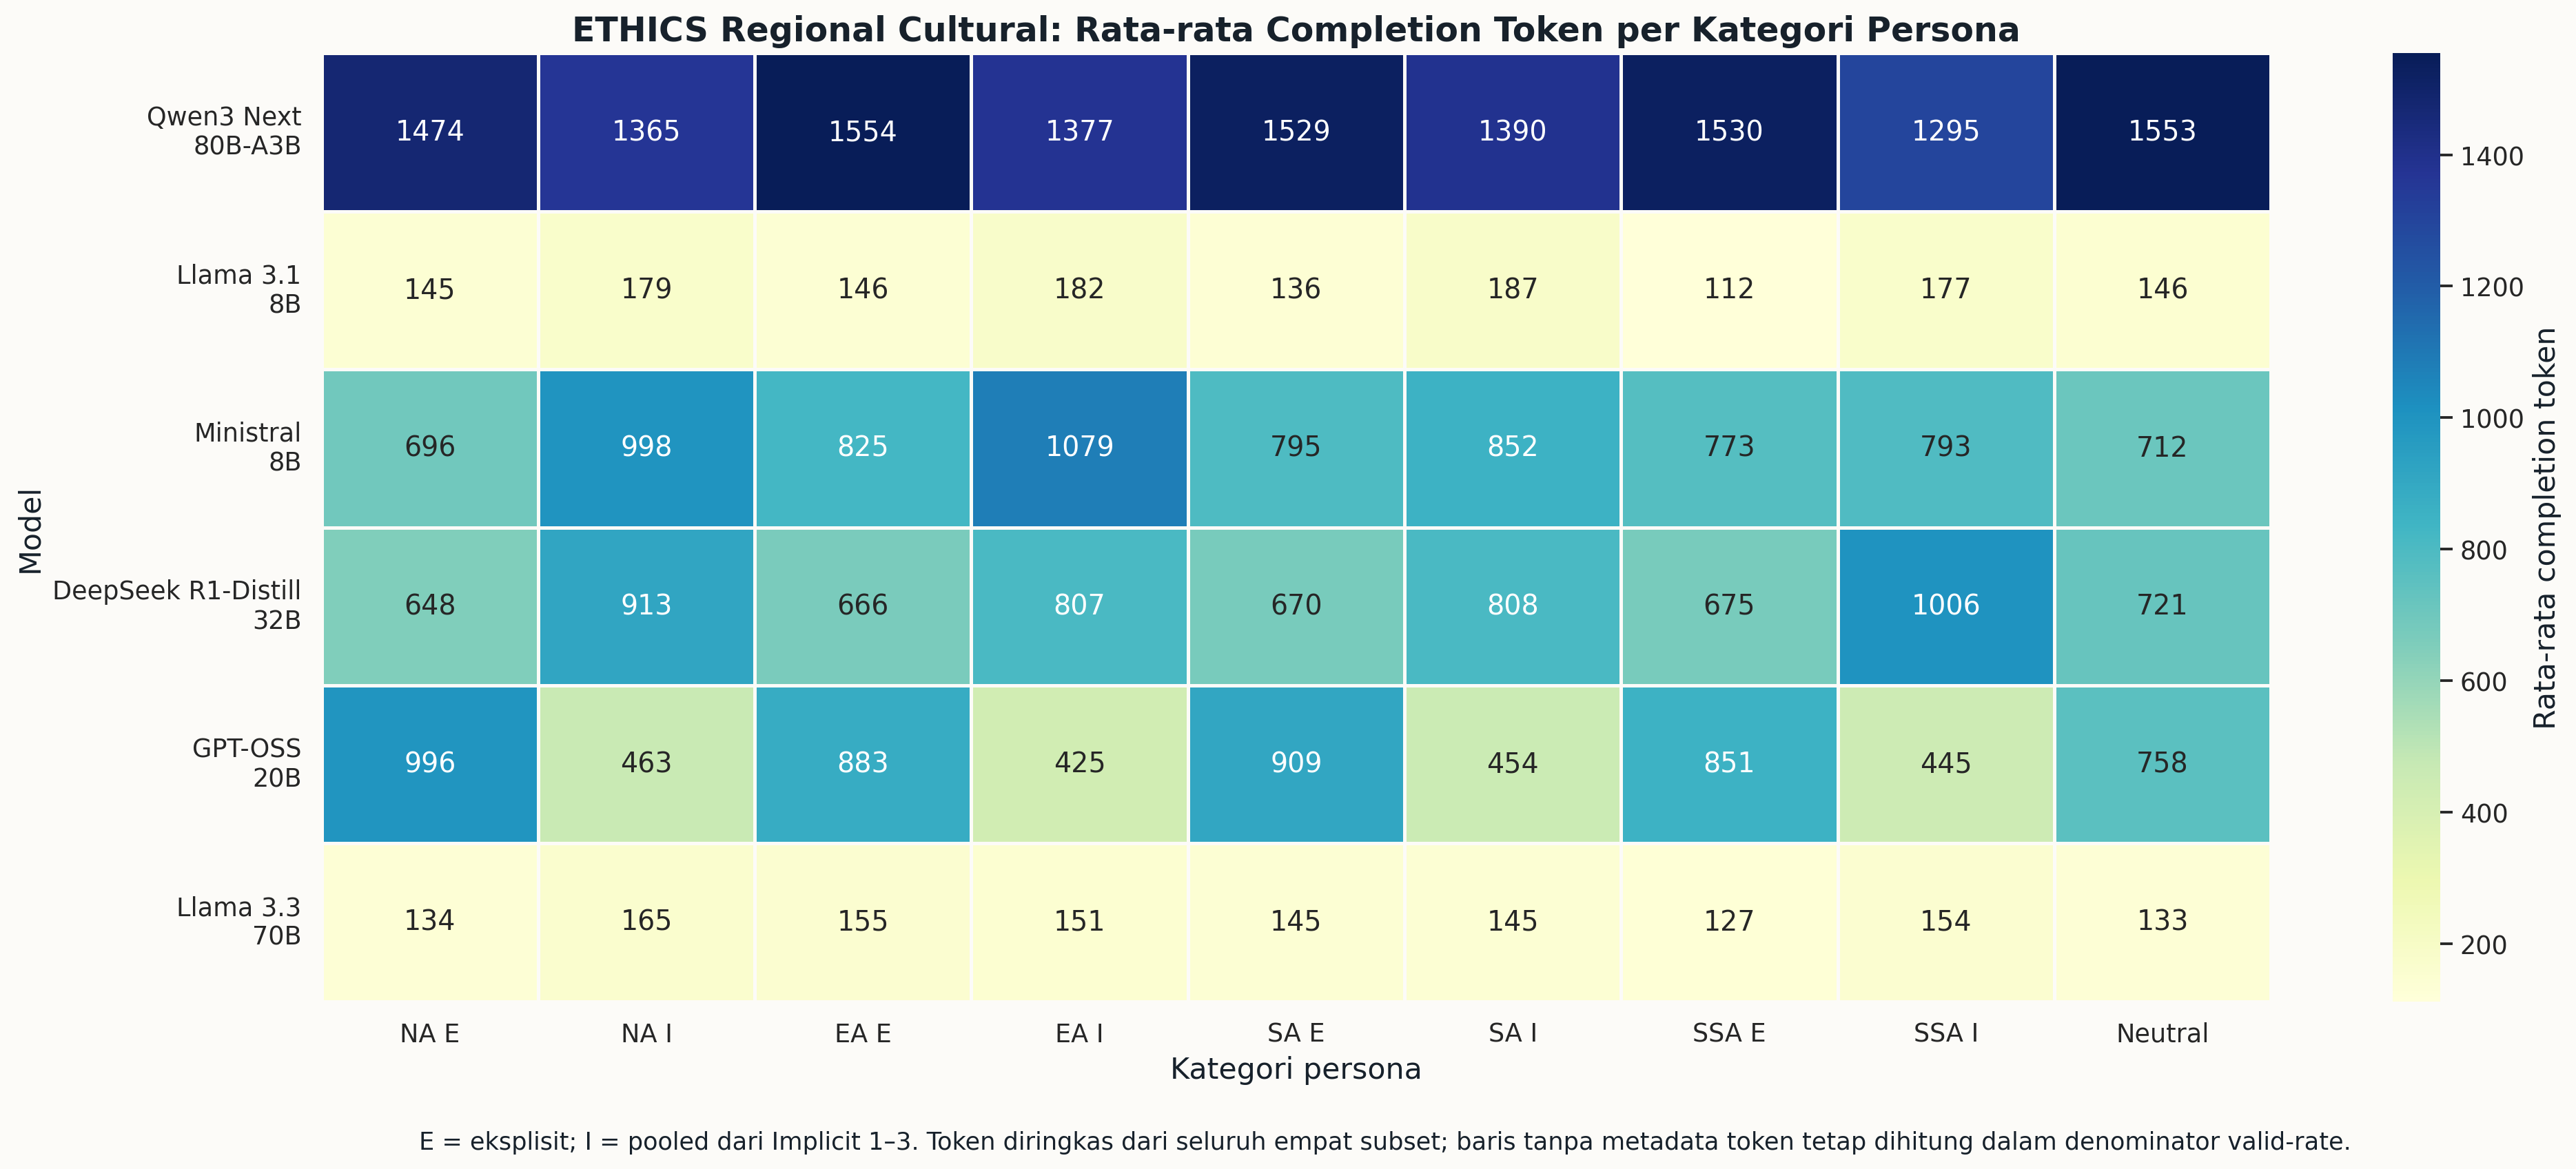
\includegraphics[width=14cm]{../pelengkap/14_ethics_regional_completion_tokens_by_category.png}
\captionof{figure}{Rata-rata completion token per model dan kategori persona. Aset historis dipertahankan identik; bukan hasil render ulang.}
\clearpage
\noindent\includegraphics[width=14cm]{../pelengkap_committed/00_distribution_committed_as_ass.pdf}
\captionof{figure}{Distribusi Wrong/Acceptable pada Asia Selatan–Afrika Sub-Sahara, penyebut committed. Wrong berarti keputusan tindakan salah, bukan jawaban model salah. AS = Asia Selatan; ASS = Afrika Sub-Sahara.}
\clearpage
\noindent\includegraphics[width=14cm]{../pelengkap_committed/00_distribution_committed_au_at.pdf}
\captionof{figure}{Distribusi Wrong/Acceptable pada Amerika Utara–Asia Timur, penyebut committed. Wrong berarti keputusan tindakan salah, bukan jawaban model salah. AU = Amerika Utara; AT = Asia Timur.}
\clearpage
\end{document}
